\Chapter{Szimulációk}

A megvalósított mesterséges intelligenciák erősségének összeméréséhez szimulációkra volt szükség. A fejezetben ezen vizsgálatok elvégzésének módját, a kapott eredményeket és értékelésüket láthatjuk.

\Section{Szimuláció program}

A szimulációk elvégzéséhez egy külön programot hoztam létre, amelyben a különböző AI-okat játszattam egymás ellen. Ezeknek a szimulációknak az eredményét kezdetben a konzolra írtam ki, hogy fel tudjam mérni a különböző AI-ok képességeit.

\SubSection{Első AI a második AI ellen}

A szimulációk elvégeztével egyértelműen látszott, hogy a második sokkal eredményesebb mint az első, hiszen általánosan körülbelül a 85\%-át tudta megnyerni a lejátszott játékoknak.

Különböző vizsgálatokat futtattam a két AI játszmáinak kapcsán. Először azt vizsgáltam, hogy milyen a lejátszott meccsek végén a játékosok összpontszámainak gyakoriság hisztogramja tízezer játék esetén (\ref{fig:scores1v2}. ábra).

\begin{figure}[h]
\centering
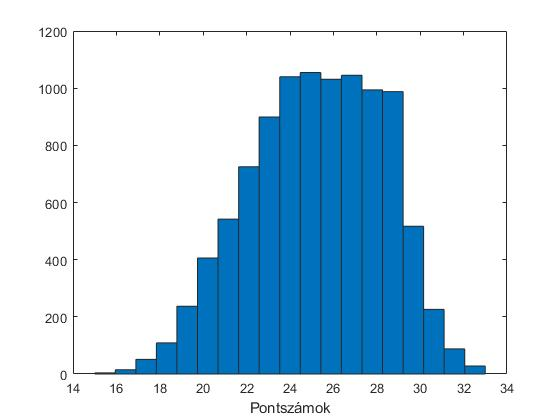
\includegraphics[scale=0.6]{images/final_scores_AI1vsAI2.jpg}
\caption{Az első és második AI összpontszámainak eloszlása.}
\label{fig:scores1v2}
\end{figure}

\newpage
Egy hasonló vizsgálat során, ugyanezen játékszám mellett a lejátszott meccsek köreinek számát tekintve vizsgáltam meg a gyakoriság hisztogramját (\ref{fig:rounds1v2}. ábra).

\begin{figure}[h]
\centering
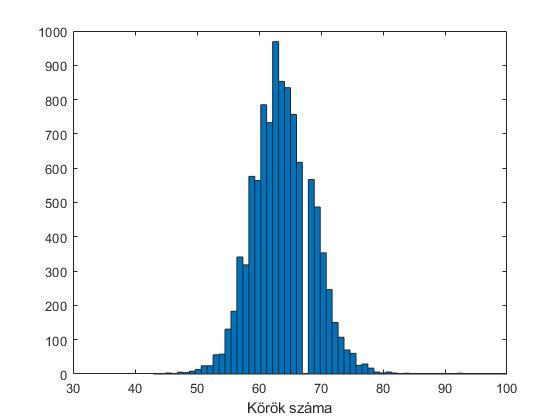
\includegraphics[scale=0.5]{images/round_number_hist_AI1vsAI2.jpg}
\caption{Az első és második AI köreinek eloszlása.}
\label{fig:rounds1v2}
\end{figure}

Végezetül pedig egy játékban a pontszámaiknak növekedését elemeztem. (\ref{fig:player_scores1v2}. ábra).

\begin{figure}[h]
\centering
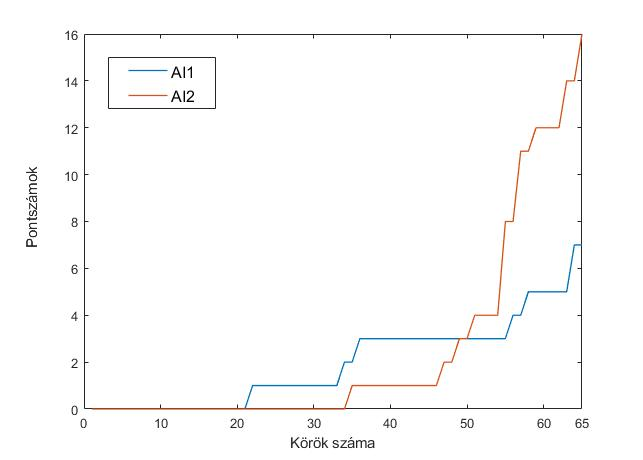
\includegraphics[scale=0.5]{images/player_points_AI1vsAI2.jpg}
\caption{Az első és második AI pontszámainak növekedése.}
\label{fig:player_scores1v2}
\end{figure}

% TODO: Ide (vagy az előző ábrák után külön-külön) kellene még valamilyen értékelés, hogy mit mutatnak az eredmények.

\SubSection{Második AI a harmadik AI ellen}

A szimulációk elvégzése után láthatóvá vált, hogy a második algoritmus nagyobb arányban tudott nyerni, mint a harmadik. Ebből az a következtetés vonható le, hogy a lapválasztást tekintve érdemesebb mindig a lehető legmagasabb szintű lapot választani a játék megnyerése érdekében. Az eredmények tekintetében a harmadik helyett továbbra is a második AI logikáját vettem alapul a következő algoritmus megvalósításakor a kártyaválasztásra nézve.

\SubSection{Második AI a negyedik AI ellen}

Ahogy elvégeztem a szimulációkat, kiderült, hogy a második logika ez esetben is nagyobb arányban tudott nyerni, mint a negyedik. Az, hogy ez az algoritmus nem hatékony abból fakad, hogy a játék előrehaladtával a késői fázisban is csak azt nézi, hogy melyik a számára legkönnyebben elérhető lap, így az alacsony szintűekre kezd el gyűjteni, nem pedig az értékesebb lapokra, így a pontszerzés szempontja a háttérbe szorul és a másik logika felé tud kerekedni.

A konklúzió, hogy a második algoritmus eredményesebb volt a harmadiktól és a negyediktől egyaránt. Ezáltal sem a kártyaválasztás, sem a zsetonválasztás terén nem sikerült előrelépni.

% TODO: Valamilyen számszerű vizsgálat ehhez a részhez is jól jöhet.

\SubSection{Második AI az ötödik AI ellen}

% TODO: Az 5. AI-t az előző fejezetben kellene bevezetni. Itt már csak értékelni kellene a kapott eredményeket.

Az ötödik AI megvalósítása során figyelembe véve az előző próbálkozások sikertelenségét, igyekeztem azokból tanulva kiküszöbölni azok buktatóit, ezáltal a kártya-, és zsetonválasztás terén egyaránt előrelépést eredményezni a másodikhoz képest.

Az AI elkészítése után lefuttatva a szimulációkat kiderült, hogy a fejlesztéseim sikeresek voltak.
Az ötödik algoritmus körülbelül annyival erősebb, mint amennyivel a második volt az elsőtől. Általánosan 86\%-kát nyeri meg a lejátszott játékaiknak. Ez bizonyult tehát a legeredményesebb logikának a szimulációim során.

Az elsőhöz hasonlóan megnéztem, hogy miként alakul a játékok végén a játékosok összpontszámainak gyakoriság hisztogramja szintén tízezer játszma esetén (\ref{fig:scores2v5}. ábra).

\begin{figure}[h]
\centering
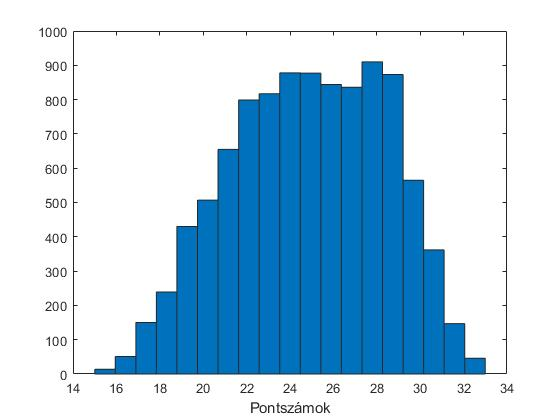
\includegraphics[scale=0.55]{images/final_scores_AI2vsAI5.jpg}
\caption{A második és ötödik AI összpontszámainak eloszlása.}
\label{fig:scores2v5}
\end{figure}

\newpage

A következő vizsgálat során tízezer játékszám mellett a lejátszott meccsek köreinek számát tekintve vizsgáltam meg a gyakoriság hisztogramját, ahogy korábban is tettem (\ref{fig:rounds2v5}. ábra).

\begin{figure}[h]
\centering
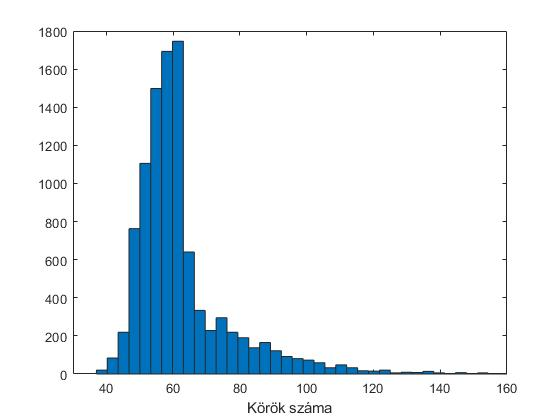
\includegraphics[scale=0.5]{images/round_number_hist_AI2vsAI5.jpg}
\caption{A második és ötödik AI köreinek eloszlása.}
\label{fig:rounds2v5}
\end{figure}

Ezután pedig az egy játékban való pontjaiknak a növekedését is szintén megvizsgáltam (\ref{fig:player_scores2v5}. ábra).

\begin{figure}[h]
\centering
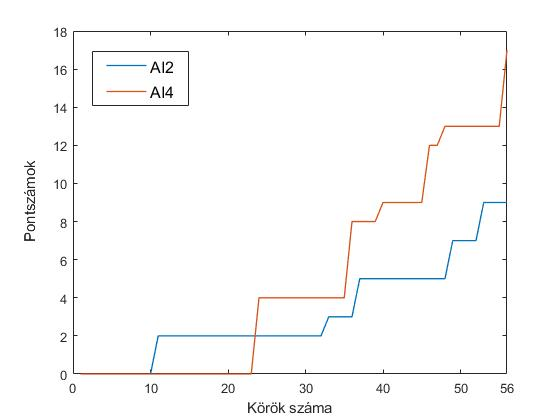
\includegraphics[scale=0.5]{images/player_points_AI2vsAI5.jpg}
\caption{A második és ötödik AI pontszámainak növekedése.}
\label{fig:player_scores2v5}
\end{figure}

% TODO: Az ábrákból itt is le kellene vonni valamilyen következtetést.

% TODO: Az eloszlásokra vonatkozóan érdekes lehet valamilyen egyszerűbb vizsgálat.

\newpage

\SubSection{Hatékonyság}

Végezetül összegyűjtöttem egy táblázatba a különböző AI-ok hatékonyságát az egymással futtatott szimulációk során. Az eredmények \aref{tab:ai_comparison}. táblázatban láthatók az eredmények, amely elkészítéséhez olyan módon módosítottam a kódomat, hogy mindig egy adott algoritmus kezdte a játékokat. A sorok mutatják, hogy melyik AI kezdett, valamint, hogy milyen százalékban tudta megnyerni a játszmákat a többivel összemérve.

\begin{table}[h]
\caption{A gépi intelligenciák eredményessége az egymás elleni szimulációkban.}
\label{tab:ai_comparison}
\medskip
\centering
\begin{tabular}{|c|c|c|c|c|c|} 
 \hline
  & AI1 & AI2 & AI3 & AI4 & AI5 \\ 
 \hline
 AI1 & 55\% & 18\% & 40\% & 22\% & 5.5\%\\ 
 \hline
 AI2 & 86\% & 56\% & 78\% & 62\% & 17\%\\ 
 \hline
 AI3 & 67\% & 30\% & 55\% & 35\% & 8.5\%\\ 
 \hline
 AI4 & 85\% & 50\% & 74\% & 56\% & 12\%\\ 
 \hline
 AI5 & 96\% & 88\% & 95\% & 92\% & 52\%\\
 \hline
\end{tabular}
\end{table}

A tesztek elvégzése után az a következtetés vonható le, hogy a körkezdésnek viszonylag nagy jelentősége van a nyerési arány tekintetében, hiszen ahogy az első algoritmusnál is láthatjuk körülbelül öt százalékkal eredményesebb volt önmagával szemben az, amelyik kezdett. Ez a randomizálás visszaszorulásával arányosan csökken, ha megnézzük az ötödik AI esetét, ahol nagyobb szerepet kap a következetesség. Ebben az esetben már csak két százalékkal volt jobb a körkezdő algoritmus.

A második és a negyedik logika erősségének összemérése esetén ez a jelenség meglepően befolyásolta az eredményt. A korábbi tesztek során kiderült, hogy a második erősebbnek bizonyult, mint a negyedik AI. Ezzel szemben azokban az esetekben, amikor a negyedik kezdett, körülbelül azonos volt a nyerési arányuk.

% TODO: Érdemes valahogy győztest választani az AI közül a táblázat eredményei alapján.
